\documentclass{beamer}

\usepackage{graphicx}
\usepackage{textpos}
\usepackage{listings}

\usetheme{Madrid}
\useoutertheme{miniframes} % Alternatively: miniframes, infolines, split

% Setup the university's color pallette
\definecolor{UIUCorange}{RGB}{19, 41, 75} % UBC Blue (primary)
\definecolor{UIUCblue}{RGB}{232, 74, 39} % UBC Grey (secondary)


\setbeamercolor{palette primary}{bg=UIUCorange,fg=white}
\setbeamercolor{palette secondary}{bg=UIUCblue,fg=white}
\setbeamercolor{palette tertiary}{bg=UIUCblue,fg=white}
\setbeamercolor{palette quaternary}{bg=UIUCblue,fg=white}
\setbeamercolor{structure}{fg=UIUCorange} % itemize, enumerate, etc
\setbeamercolor{section in toc}{fg=UIUCblue} % TOC sections

\setbeamercolor{subsection in head/foot}{bg=UIUCorange,fg=UIUCblue}
\setbeamercolor{subsection in head/foot}{bg=UIUCorange,fg=UIUCblue}

\usepackage[utf8]{inputenc}
\usepackage{graphicx}


%Information to be included in the title page:
\title{\textbf{Introduction to the Course}}
\author{\textbf{David H Smith IV}}
\institute[\textbf{UIUC}]{\textbf{University of Illinois Urbana-Champaign}}
\date{\textbf{Mon, June 14 2021}}

\setbeamertemplate{title page}[default][colsep=-4bp,rounded=true]
\addtobeamertemplate{title page}{\vspace{3\baselineskip}}{}
\addtobeamertemplate{title page}{
  \begin{textblock*}{\paperwidth}(-1.0em, -1.2em)
    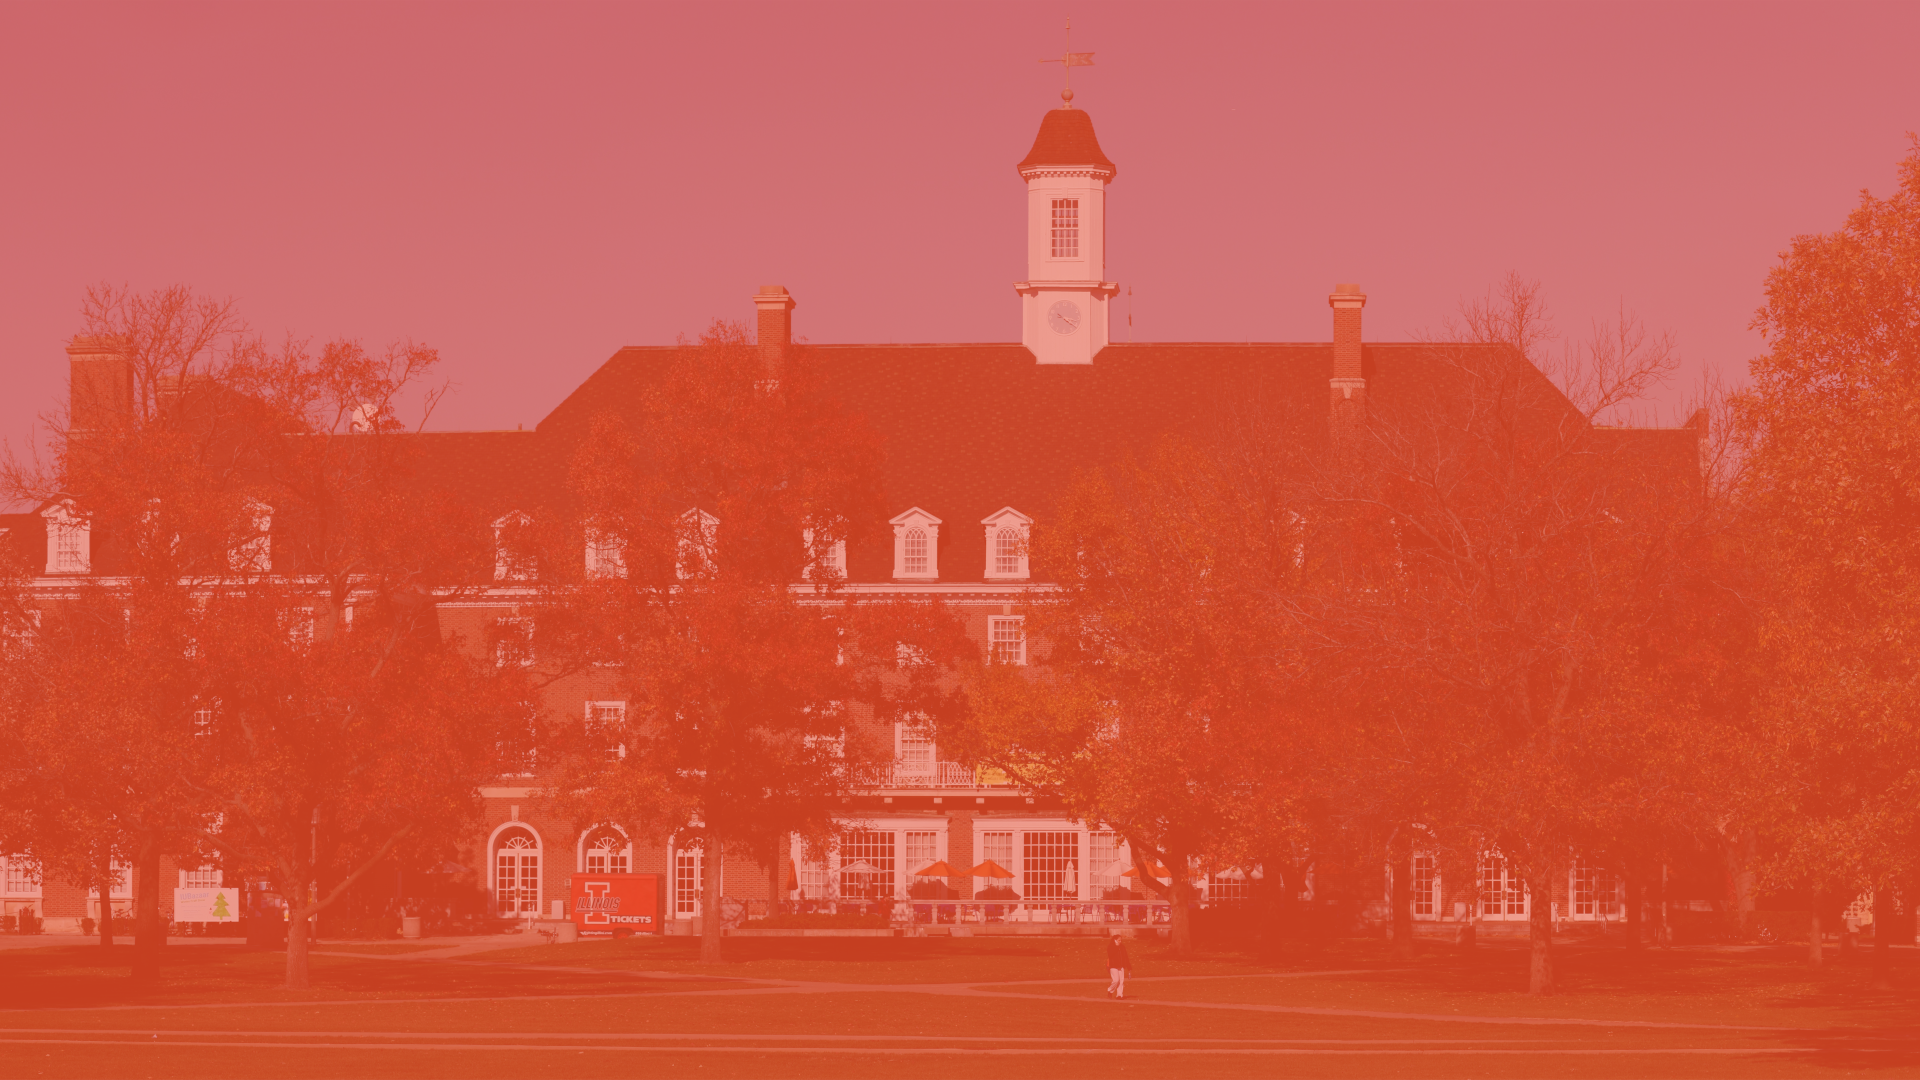
\includegraphics[width=\paperwidth, height=\paperheight]{imgs/uiuc.png}
  \end{textblock*} 
}{}

\begin{document}

\frame{\titlepage}

\section{Course Overview}

%
% Slide 1
%
\begin{frame}
  \frametitle{Course Outcomes}
  \begin{itemize}
    \item Given a small section of code you should be able to:
      \begin{itemize}
        \item Trace through and predict it's output.
        \item Describe, in plain English, what it does.
      \end{itemize}
    \item Write a small python program some, or all, of the fundamentals you will learn in the course.
    \item Beginner and intermediate spreadsheet operations.
    \item Beginner level understanding of how the internet works and how to write basic HTML documents.
  \end{itemize}
\end{frame}

\section{Overview and History of Computer Science}

%
% Slide 2
%
\begin{frame}
  \frametitle{What is Computer Science?}
  \begin{itemize}
    \item CS is concerned with understanding:
      \begin{itemize}
        %\pause
      \item What is computable
        %\pause
      \item How to compute it in one or more of the following in mind:
        \begin{itemize}
          %\pause
        \item Speed
          %\pause
        \item Reliability
          %\pause
        \item Security 
          %\pause
        \item Resource cost
      \end{itemize}
      %\pause
  \end{itemize}
  \end{itemize}
\end{frame}


%
% Slide 3
%
\begin{frame}
  \frametitle{What is Programming?}
  \begin{minipage}{0.5\textwidth}
    \begin{itemize}
      \item Programming $\neq$ Computer Science
        \begin{itemize}
          \item Rather, programming is a subset of Computer Science
        \end{itemize}
        %\pause
      \item ``Computer Science is no more about computers than astronomy is about telescopes'' - Edsger W. Dijkstra
        \begin{itemize}
          \item A bit of an overstatement but still a useful thing to keep in mind.
        \end{itemize}
        %\pause
      \item \textbf{High Level Definition: } A series of instructions that a computer carries out.
    \end{itemize}
  \end{minipage}
  \begin{minipage}{0.5\textwidth}
  \end{minipage}
\end{frame}

%
% Slide 4
%
\begin{frame}
  \frametitle{Where did this all come from?}
\end{frame}

%
% Slide 5
%
\begin{frame}
  \frametitle{Early ``Computers''}
  \begin{minipage}{0.59\textwidth}
  \end{minipage}
  \begin{minipage}{0.39\textwidth}
  \end{minipage}
\end{frame}

%
% Slide 6
%
\begin{frame}
  \frametitle{The Difference Engine}
  \begin{minipage}{0.59\textwidth}
  \end{minipage}
  \begin{minipage}{0.39\textwidth}
    \begin{figure}
      \label{fig:analyticalengine.png}
    \end{figure}
    \begin{figure}
      \label{fig:adababage.png}
    \end{figure}
  \end{minipage}
\end{frame}

%
% Slide 7
%
\begin{frame}
  \frametitle{Alan Turing, Alonzo Church, and Turing Machines}
  \begin{minipage}{0.59\textwidth}
    \begin{enumerate}
      \item \textbf{Church-Turing Thesis} - Any effective calculation can be performed by a mechanical computer (e.g., a Turing Machine).
      \item \textbf{Turing Machines} - An abstract, mathematical model of a machine that moves up and down a strip of paper, one step at a time, and performs operations based on a set of rules (Figure \ref{fig:turingmachine}).
    \end{enumerate}
  \end{minipage}
  \begin{minipage}{0.39\textwidth}
    \begin{figure}
      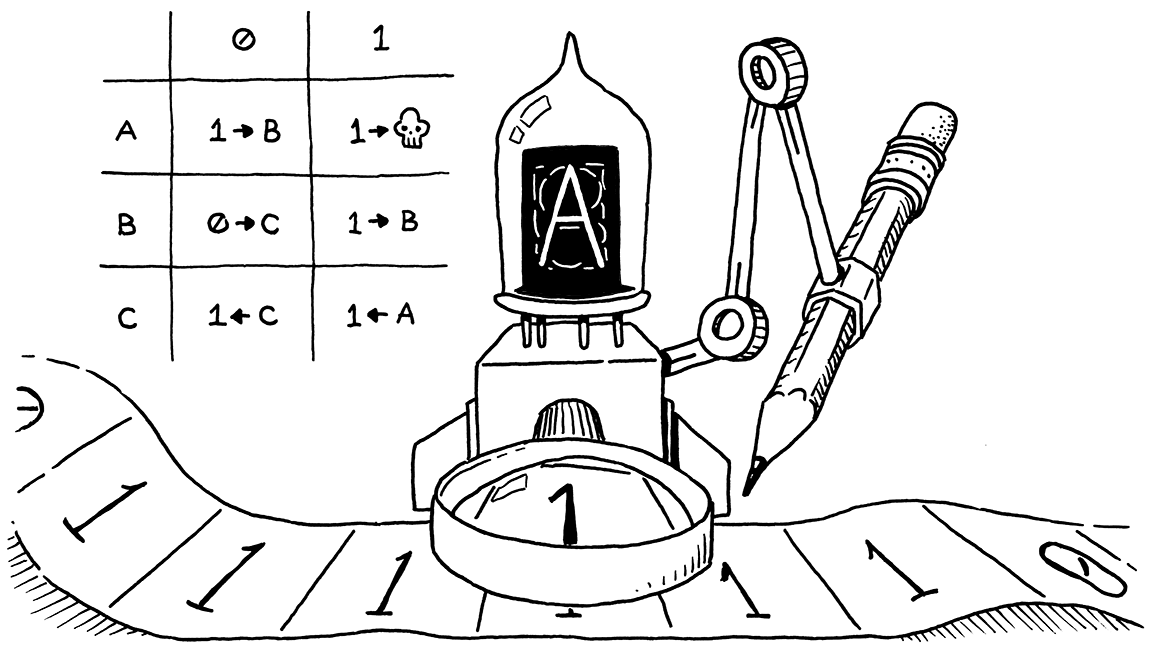
\includegraphics[width=\textwidth]{imgs/turing-machine.png}
      \caption{Artists Representation of a Turing Machine}
      \label{fig:turingmachine}
    \end{figure}
  \end{minipage}
\end{frame}

%
% Slide 9
%
\begin{frame}
  \frametitle{Von Neumann Architecture}
  \begin{minipage}{0.59\textwidth}
    \begin{enumerate}
      \item \textbf{Input Devices: } Something with buttons and knobs.
        %\pause
      \item \textbf{Central Processing Unit:}
        \begin{enumerate}
          \item \textbf{Control Unit: } Manages other parts.
          \item \textbf{Arithmetic/Logic Unit: } Does math on integers.
        \end{enumerate}
        %\pause
      \item \textbf{Memory Unit: } Supplies info to CPU (i.e., Random Access Memory).
        %\pause
      \item \textbf{External Storage Unit (Not Pictured): } We often need larger storage for data that isn't needed immediately (e.g., Hard Drive).
        %\pause
      \item \textbf{Output Devices: } Flashing lights, monitor, etc.
    \end{enumerate}
  \end{minipage}
  \begin{minipage}{0.39\textwidth}
    \begin{figure}
      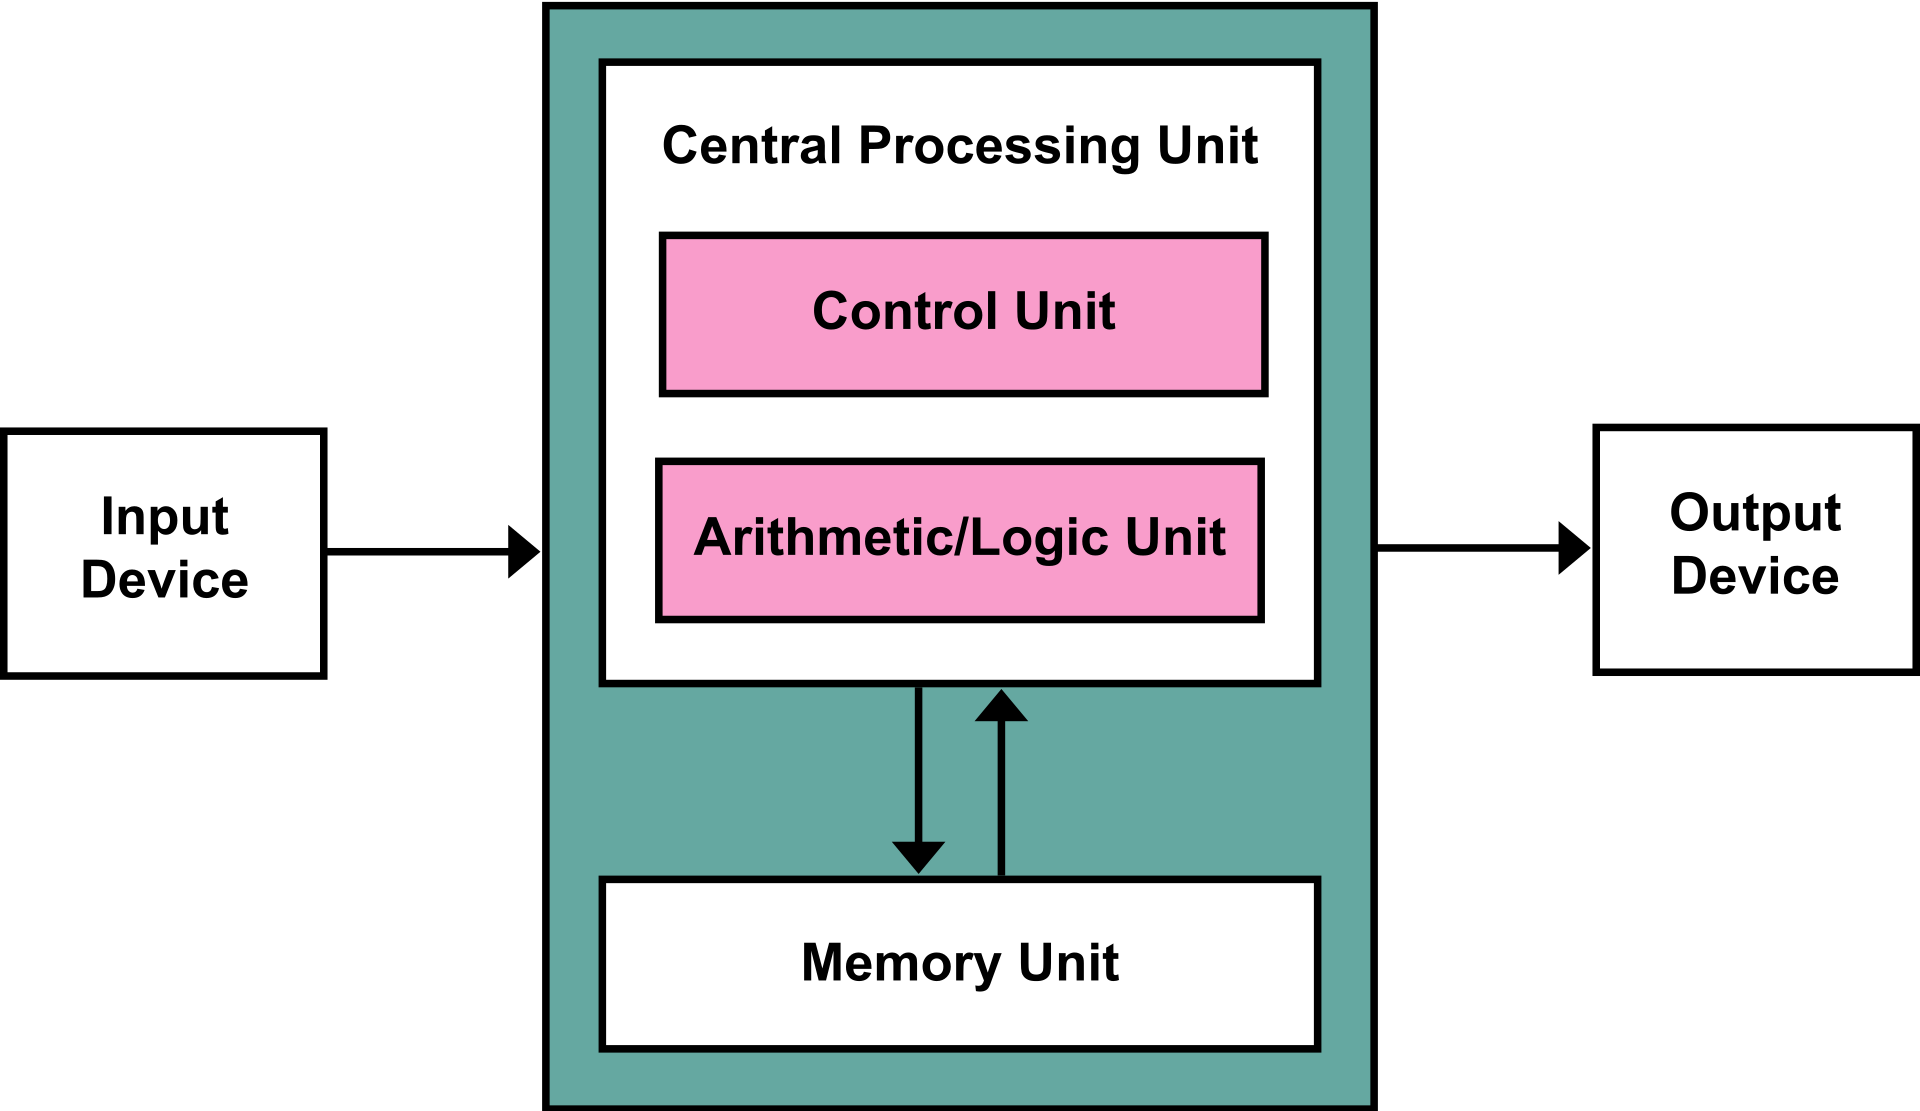
\includegraphics[width=\textwidth]{imgs/von-neumann-arch.png}
      \caption{Von Neumann Architecture}
      \label{fig:vonneumannarch}
    \end{figure}
  \end{minipage}
\end{frame}

%
%
%
\begin{frame}
  \frametitle{}
\end{frame}

%
% Slide 10
%
\section{Break}
\begin{frame}
  \frametitle{Break time!}
  \centering
  \Huge 5 Minute Break
\end{frame}

\section{Input, Output, and Variables}

%
% Slide 9
%
\begin{frame}
  \frametitle{Computers Run Low-Level Instructions}
  \begin{minipage}{0.75\textwidth}
    \begin{itemize}
      \item Computers don't ``Play a video''
      \item They\ldots
        \begin{enumerate}
          \item Move some numbers into memory.
          \item Do some math, or a comparison, or both
          \item Make a decision based on the results
          \item Rise a and repeat a few million time before something useful happens
        \end{enumerate}
      \item Programming at this level is:
        \begin{itemize}
          \item Tedious and error prone.
          \item Needs \textbf{\textit{A LOT}} of code to do anything useful.
          \item Isn't portable. Each processor is it's own machine and will require a different set of instructions that works with it's parts.
        \end{itemize}
    \end{itemize}
  \end{minipage}
  \begin{minipage}{0.75\textwidth}
  \end{minipage}
\end{frame}

%
% Slide 10
%
\begin{frame}
  \frametitle{Enter Python (And Other High-Level Languages)}
  \begin{itemize}
    \item They are:
      \begin{itemize}
        \item \textbf{Productive} \textrightarrow A few lines do a lot and it's easy to debug.
          %\pause 
        \item \textbf{Safer} \textrightarrow Less likely to write code that is insecure or damaging.
          %\pause 
        \item \textbf{Portable} \textrightarrow Works on all systems that support the Python interpreter.
      \end{itemize}
    \item Used for everything from machine learning to general scripting.
      %\pause 
    \item We use Python 3.x (not Python 2.x)
  \end{itemize}
\end{frame}

\begin{frame}
  \frametitle{How programs are Constructed}
  \begin{itemize}
    \item \textbf{Algorithms} \textrightarrow A step-by-step process for achieving a result
      \begin{itemize}
        \item Often Written in pseudo-code
      \end{itemize}
    \item \textbf{Programming} \textrightarrow Express the commands in a form the computer understands.
  \item \textbf{Testing} \textrightarrow Designing inputs that test specific behaviours of the code.
  \item \textbf{Debugging} \textrightarrow Finding errors in the code based on the results of your tests and fixing them.
  \end{itemize}
\end{frame}


\begin{frame}
  \frmaetitle{How Languages are Constructed}
  \begin{itemize}
    \item \textbf{Syntax} \textrightarrow Rules of how programs should be constructed (think grammar).
    \item \textbf{Semantics} \textrightarrow Rules specifying what a program does.
  \end{itemize}
\end{frame}


%
% Slide 11
%
\begin{frame}
  \frametitle{Data Types in Python}
  \begin{itemize}
    \item Two types we'll need to know now:
      \begin{itemize}
        \item \textbf{Strings: } A long list of characters accompanied by surrounding quotes (e.g., ``Hello, CS 105!'').
        \item \textbf{Integers: } Whole numbers, both positive and negative.
      \end{itemize}
    \item You can check the type of a variable or expression with the \lstinline{type()} function.
    %\pause
    \item You can convert between them with the \lstinline{str()} and \lstinline{int()} functions.
    %\pause
    \item It's important to keep the type of your variables in mind when programming.
    %\pause
    \item Keeping types in mind when attempting to deduce what a program is doing is very important. 
  \end{itemize}
\end{frame}


%
% Slide 12
%
\begin{frame}
  \frametitle{Poll Question: Python Values have Types}
  \centering
  \Huge
  What is the type of x if x is assigned x = 23?
\end{frame}


%
% Slide 11
%
\begin{frame}
  \frametitle{Input and Print}
  \begin{itemize}
    \item \underline{\textbf{The Input Function}}: A builtin function that gets a string from the user.
      %\pause
      \begin{itemize}
        \item \textbf{input()} \textrightarrow Doesn't give a prompt.
      %\pause
        \item \textbf{input(``A test input: '')} \textrightarrow Will output the message \textit{"A test input:"} to the screen and let the user type their input in after it.
      %\pause
      \end{itemize}
    \item \underline{\textbf{The Print Function}}: A builtin function that takes a string as a parameter (in between the parentheses) and outputs that string
      %\pause
      \begin{itemize}
        \item \textbf{print(``Hello, World!'')} \textrightarrow Will output the ``Hello, World!''. 
      \end{itemize}
  \end{itemize}
\end{frame}

%
% Slide 12
%
\begin{frame}
  \frametitle{Poll Question: Input and Print}
  Assuming there is a variable value with the value 7, which of the following statements prints: count = 7.
  \begin{enumerate}
    \item \lstinline{print("count = " value)}
    \item \lstinline{print("count = ", end="value")}
    \item \lstinline{print("count = ", value)}
    \item \lstinline{print("count = \$value")}
  \end{enumerate}
\end{frame}


\section{Acknowledgements}


\begin{frame}
  \begin{enumerate}
    \item
  \end{enumerate}
\end{frame}


\end{document}
